\documentclass{standalone}

\renewcommand{\familydefault}{\sfdefault}
\usepackage{amsmath}
\usepackage{tikz}
\usetikzlibrary{arrows.meta, positioning, calc, }

\begin{document}

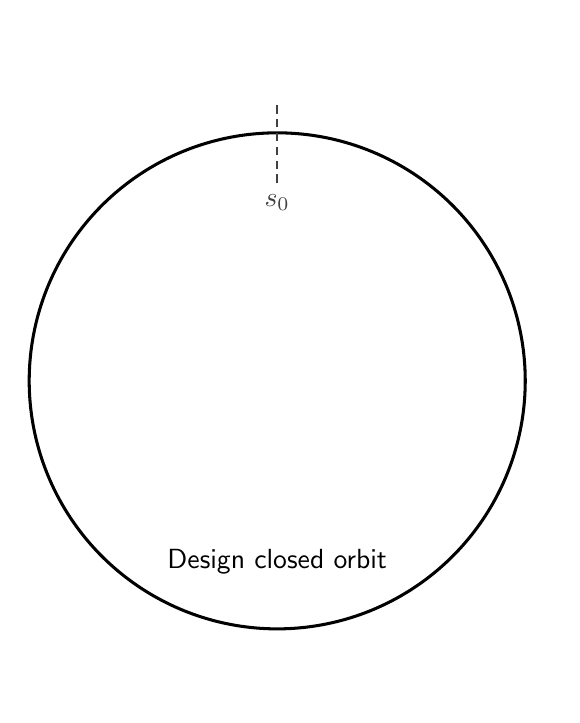
\begin{tikzpicture}[>=latex]
    % a orbita fechada ideal/desing
    % \draw[black, thick] (0, 0) circle (3.1);
    \draw[domain=0:360, variable=\t, samples=500, black, line width=1.1pt, scale=3.15] plot (
    {sin(\t)}, 
    {cos(\t)});

    % \draw[->] (-4, 0) -- (4, 0) node[right] {$x$};
    % \draw[->] (0, -4) -- (0, 4) node[right] {$y$};

    \draw[densely dashed, darkgray, line width=0.8pt] (0, 3.5) -- (0, 2.5) node[below] {$s_0$};

    \node[black] at (0, -2.3) {Design closed orbit};

    \node[above, opacity=0] at (0, 4) {Kick};
    \node[opacity=0, below right] at (0, -3.5) {Perturbed closed orbit};


\end{tikzpicture}


\end{document}
